\documentclass[10pt]{article}
\usepackage[utf8]{inputenc}
\usepackage{parskip}
\usepackage[margin = 1in]{geometry}
\usepackage{xcolor}
\usepackage[colorlinks = true,linkcolor = blue, urlcolor  = blue,citecolor = blue,anchorcolor = blue]{hyperref}
\usepackage{framed}
\usepackage{apacite}
\usepackage[authoryear,sort]{natbib}
\usepackage{amsmath}
\bibliographystyle{apalike}
\newcommand{\E}{\textrm{E}}
\renewcommand*{\theenumi}{\thesection.\arabic{enumi}}
\usepackage{tikz}
\usetikzlibrary{arrows,shapes.arrows,positioning,shapes,patterns,calc}

\begin{document}

\begin{Large} 
Info 6751. Fall 2022. Problem Set 3. Due on Canvas by 5pm on 12 Sep.
\end{Large}
\hline

\section{(32 points) Material covered Tuesday}
Part 1 is about the \textbf{Directed Acyclic Graphs (DAGs)}.

For 1.1--1.5, answer True or False: $X$ is a sufficient adjustment set to identify the causal effect of $A$ on $Y$. Explain in one sentence. If False, state the backdoor path that is unblocked conditional on $X$.

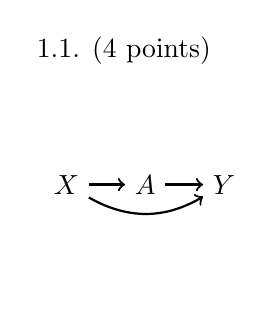
\begin{tikzpicture}
    \node[anchor = north west] at (-1.5,2) {1.1. (4 points)};
    \node (x) at (-1,0) {$X$};
    \node (a) at (0,0) {$A$};
    \node (y) at (1,0) {$Y$};
    \draw[->, thick] (a) -- (y);
    \draw[->, thick] (x) -- (a);
    \draw[->, thick] (x) to[bend right] (y);
    \node at (0,-1.2) {};
\end{tikzpicture}
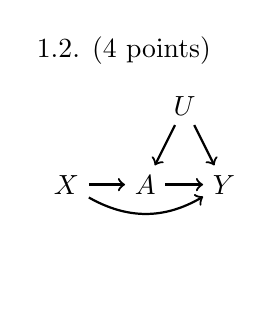
\begin{tikzpicture}
    \node[anchor = north west] at (-1.5,2) {1.2.  (4 points)};
    \node (x) at (-1,0) {$X$};
    \node (a) at (0,0) {$A$};
    \node (y) at (1,0) {$Y$};
    \draw[->, thick] (a) -- (y);
    \draw[->, thick] (x) -- (a);
    \draw[->, thick] (x) to[bend right] (y);
    \node (u1) at (.5,1) {$U$};
    \draw[->, thick] (u1) -- (a);
    \draw[->, thick] (u1) -- (y);
    \node at (0,-1.2) {};
\end{tikzpicture}
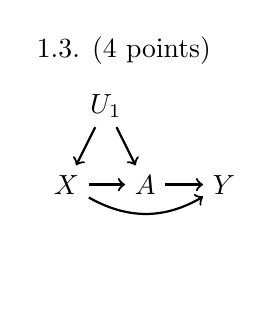
\begin{tikzpicture}
    \node[anchor = north west] at (-1.5,2) {1.3. (4 points)};
    \node (x) at (-1,0) {$X$};
    \node (a) at (0,0) {$A$};
    \node (y) at (1,0) {$Y$};
    \draw[->, thick] (a) -- (y);
    \draw[->, thick] (x) -- (a);
    \draw[->, thick] (x) to[bend right] (y);
    \node (u1) at (-.5,1) {$U_1$};
    \draw[->, thick] (u1) -- (x);
    \draw[->, thick] (u1) -- (a);
    \node at (0,-1.2) {};
\end{tikzpicture}
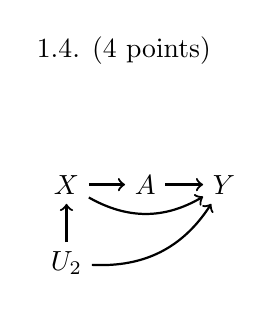
\begin{tikzpicture}
    \node[anchor = north west] at (-1.5,2) {1.4. (4 points)};
    \node (x) at (-1,0) {$X$};
    \node (a) at (0,0) {$A$};
    \node (y) at (1,0) {$Y$};
    \draw[->, thick] (a) -- (y);
    \draw[->, thick] (x) -- (a);
    \draw[->, thick] (x) to[bend right] (y);
    \node (u2) at (-1,-1) {$U_2$};
    \draw[->, thick] (u2) -- (x);
    \draw[->, thick] (u2) to[bend right] (y);
    \node at (0,-1.2) {};
\end{tikzpicture}
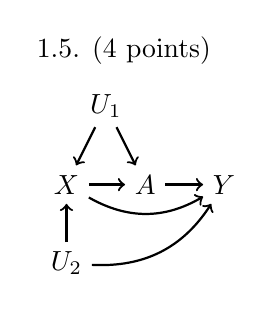
\begin{tikzpicture}
    \node[anchor = north west] at (-1.5,2) {1.5. (4 points)};
    \node (x) at (-1,0) {$X$};
    \node (a) at (0,0) {$A$};
    \node (y) at (1,0) {$Y$};
    \draw[->, thick] (a) -- (y);
    \draw[->, thick] (x) -- (a);
    \draw[->, thick] (x) to[bend right] (y);
    \node (u1) at (-.5,1) {$U_1$};
    \draw[->, thick] (u1) -- (x);
    \draw[->, thick] (u1) -- (a);
    \node (u2) at (-1,-1) {$U_2$};
    \draw[->, thick] (u2) -- (x);
    \draw[->, thick] (u2) to[bend right] (y);
    \node at (0,-1.2) {};
\end{tikzpicture}

For each statement below, answer True or False. Explain in one sentence.
\begin{enumerate}
    \setcounter{enumi}{5}
    \item (4 points) Conditioning on $X$ blocks this path: $A\leftarrow B \leftarrow X \rightarrow C \rightarrow Y$
    \item (4 points) Conditioning on $X$ blocks this path: $A\leftarrow B \rightarrow X \leftarrow C \rightarrow Y$
\end{enumerate}

For the scenario below, draw a DAG with a counterexample. Explain to the researcher why this algorithm could produce misleading results.
\begin{enumerate}
    \setcounter{enumi}{7}
    \item (4 points) A researcher comes to you with a new machine learning method. It uses LASSO to search for variables that are predictive of both the treatment $A$ and the outcome $Y$, and it includes in the model the union of those sets. 
\end{enumerate}


\section{(18 points) Material covered Thursday}
Part 2 is all about the \textbf{population inference}.

A researcher uses an opt-in online web survey to draw inference about support for President Biden. They ask respondents: ``Do you approve of President Biden's performance in office?'' with the answer choices Yes/No. The researcher also gathers data on several demographic characteristics: race, whether the respondent completed college, and annual family income. They write:
\begin{quote}
    The distribution of race, college, and income in my sample matches the distribution I estimate in the American Community Survey, a national probability sample collected by the Census Bureau. Therefore, my sample-based evidence about support for President Biden generalizes to the population.
\end{quote}
This question is about formalizing a set of conditions under which the researcher is right and wrong. Assume throughout that the Census Bureau estimates are correct.

\begin{enumerate}
    \item (5 points) Draw a DAG under which the researcher's claim is valid. Use $S$ as a random variable indicating inclusion in the sample.
    \item (3 points) In a sentence or two, explain your DAG from 2.1 to the researcher.
    \item (5 points) Draw a DAG showing a counterexample under which the researcher's claim is invalid. Use $S$ as a random variable indicating inclusion in the sample.
    \item (3 points) In a sentence or two, explain your DAG from 2.3 to the researcher.
    \item (2 points) One researcher does the above procedure with a sample of $n = 100$. Another researcher does the above procedure with a sample of $n = 1,000$. Does the size of the sample affect the validity of population inference?
\end{enumerate}

\end{document}
